\section{Methodology}
\label{sec:methodology}
The current repository implements a proof-of-concept generative workflow built from four components: a noise scheduler, a latent diffusion-style denoiser, a latent-to-3D converter, and an internal CFD-oriented evaluator. The codebase now has two evidence tracks: deterministic synthetic/procedural smoke data retained for continuity, and a public VSP Airshow corpus used for the grounded training smoke run reported in Section \ref{sec:results}. In this revision, the same path also carries a documented structured condition vector through dataset generation, latent construction, and checkpointed inference. Figure \ref{fig:architecture} should therefore be read as an implementation diagram for the present repository rather than as evidence of a fully validated aircraft-design system.

\begin{figure*}[!t]
\centering
\begin{tikzpicture}[
    node distance=0.55cm and 0.65cm,
    stage/.style={draw, rounded corners=2pt, align=center, minimum height=0.78cm, text width=2.15cm, font=\footnotesize},
    evidence/.style={draw, dashed, rounded corners=2pt, align=center, minimum height=0.7cm, text width=2.55cm, font=\scriptsize},
    arrow/.style={->, thick}
]
\node[stage] (latent) {Latent sample\\and condition vector};
\node[stage, right=of latent] (denoise) {Latent diffusion-style\\denoiser};
\node[stage, right=of denoise] (decode) {Voxel decoder\\and cleanup};
\node[stage, right=of decode] (score) {Internal CFD-oriented\\scoring path};
\node[stage, right=of score] (export) {STL and OpenFOAM\\export route};

\node[evidence, below=of denoise] (smoke) {Evidence today:\\reduced protocol gates};
\node[evidence, below=of score] (future) {Future gates:\\structural and\\CFD validation};

\draw[arrow] (latent) -- (denoise);
\draw[arrow] (denoise) -- (decode);
\draw[arrow] (decode) -- (score);
\draw[arrow] (score) -- (export);
\draw[arrow] (decode) -- (smoke);
\draw[arrow] (score) -- (future);
\end{tikzpicture}
\caption{Implementation-level view of the current repository. A latent code and optional structured condition vector are routed through denoising, voxel decoding, cleanup, internal scoring, and export paths. The diagram describes the code path under test; it does not by itself establish differentiable training, structural viability, or publication-grade CFD validation.}
\label{fig:architecture}
\end{figure*}

\subsection{Public Airshow Corpus Construction}
The grounded corpus path collects public model documents from the VSP Airshow web app, keeps only records whose Airshow license identifiers map to CC0, CC BY, or CC BY-SA, and requires a public preview-geometry URL before a record can enter the training manifest \cite{openvspGithub,openvspLicense,vspAirshow}. The builder parses available X3D indexed-face-set geometry, normalizes each mesh into a centered unit cube, voxelizes the occupied geometry into a fixed grid, and records source URLs, license metadata, geometry hashes, voxel hashes, split assignment, and preprocessing provenance. The primary smoke run uses a \(16^3\) grid, and the later resolution addendum reruns the same corpus construction at \(32^3\), \(64^3\), and \(96^3\). The deterministic split assignment is stored in the manifest so that later validation, training, and generation commands can be tied back to the same corpus lineage.

\begin{figure*}[!t]
\centering
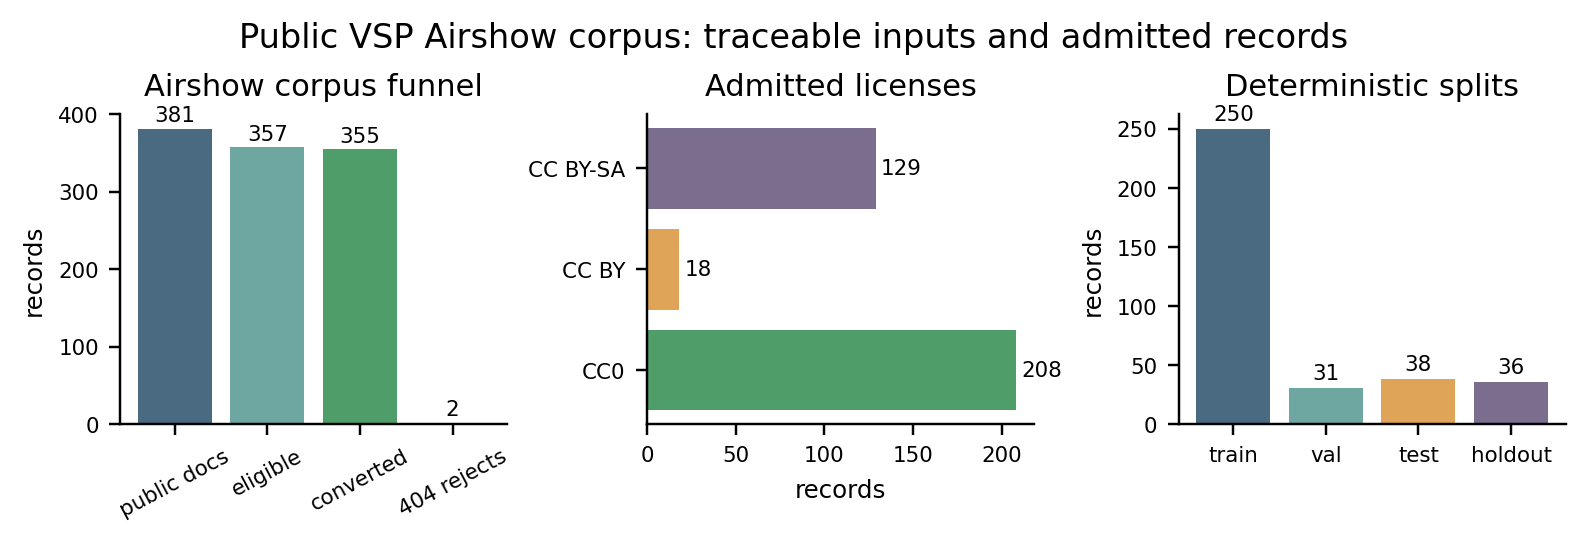
\includegraphics[width=0.94\textwidth]{figures/airshow_corpus_summary.png}
\caption{Corpus construction summary for the public VSP Airshow smoke run. The plot shows the observed Airshow model-document count, license-and-geometry filtering, converted voxel records, admitted license mix, and deterministic train/validation/test/holdout split. These counts document data provenance and coverage; they do not certify manufacturer approval or aircraft performance.}
\label{fig:airshow_corpus_summary}
\end{figure*}

The run used in this paper observed 381 public Airshow model documents, admitted 357 license-and-geometry-eligible documents, and converted 355 records after two public storage URLs returned 404. Figure \ref{fig:airshow_corpus_summary} visualizes that corpus funnel together with the license and split distributions. Airshow model names, manufacturer fields, URLs, and license labels are treated as source metadata only. The additional mission and manufacturing fields used by the condition vector are deterministic repository inferences from geometry and defaults, not factual claims made by NASA, Lockheed, OpenVSP, or any other named source.

\subsection{Noise Scheduling}
The forward diffusion process gradually adds Gaussian noise to the input data over a series of T timesteps. The noise schedule is defined by a variance schedule $\beta_t$, which is typically a linear or cosine schedule. The implementation uses a linear schedule, where $\beta_t$ increases linearly from $\beta_{start}$ to $\beta_{end}$.

The forward process is defined as:
\begin{equation}
q(x_t | x_{t-1}) = \mathcal{N}(x_t; \sqrt{1 - \beta_t} x_{t-1}, \beta_t I)
\end{equation}

During reverse sampling, the denoiser estimates the noise component of a noisy latent. The training loss compares predicted noise with sampled noise; sampling then uses that estimate to update the latent.

\subsection{Latent Diffusion UNet}
The denoising model is a UNet-based architecture that operates in the latent space. The UNet takes as input a noisy latent vector, a timestep embedding, and an optional condition embedding, and outputs the predicted noise. The implementation projects the latent to a small spatial tensor and applies residual block stacks with additive skip connections. The skip path is intended to preserve intermediate spatial features during denoising.

\subsection{Latent-to-3D Converter}
The latent-to-3D converter maps the denoised latent vector to voxel logits. For lower-resolution smoke runs, this is a dense multi-layer perceptron (MLP) whose final layer emits the whole voxel grid. For the \(96^3\) follow-up, the implementation switches to a coordinate decoder that evaluates an MLP over the latent vector concatenated with normalized \((z,y,x)\) coordinates; training samples voxel coordinates with importance-weighted BCE so occupied coordinates can be oversampled without changing the intended sparse reconstruction objective. Downstream training and generation code applies a sigmoid to convert logits into voxel probabilities.

\subsection{CFD Simulator}
The repository uses an internal lattice-Boltzmann-style CFD evaluator to score generated voxel grids. The evaluator takes a voxel geometry and flow settings such as Mach number or Reynolds number and returns drag- and lift-related quantities. In addition, the repository can export benchmark cases for comparison against an external OpenFOAM run. This combination is useful for code-path validation, but the present paper does not treat it as a substitute for a full aerodynamic validation campaign.

\subsection{Loss Function}
A simplified view of the current training objective distinguishes the base differentiable model losses from the measured solver-in-loop term. The optimizer step uses diffusion, decoded-geometry reconstruction, direct generation reconstruction, consistency, and, when scheduled, a direct internal-solver objective:

\begin{equation}
\mathcal{L}_{opt} =
\mathcal{L}_{diff}
+ \lambda_{geom}\mathcal{L}_{geom}
+ \lambda_{gen}\mathcal{L}_{gen}
+ \mathcal{L}_{cons}
+ \lambda_{solver}\mathcal{L}_{solver\mbox{-}SPSA}.
\end{equation}

The diffusion loss is the mean squared error between the predicted noise and the actual noise. The decoded-geometry and generation-reconstruction terms compare voxel logits against the target voxel grid, while the consistency term supports the reduced-step sampler. The solver term materializes voxel probabilities into a full grid, converts them to a binary geometry by thresholding or top-k occupancy selection, calls the internal D3Q27 lattice-Boltzmann evaluator on that geometry, and combines the measured aerodynamic score with an optional exact connected-component penalty. This path is not a learned stand-in: the scalar used in \(\mathcal{L}_{solver\mbox{-}SPSA}\) comes from solver calls made during training.

The connected-component operation, binary materialization step, and internal CFD evaluator are not ordinary PyTorch operations with analytic gradients. The training loop therefore uses a two-sided simultaneous perturbation estimate when this term is active. For a probability grid \(V\), a perturbation field \(\Delta\), and perturbation scale \(\epsilon\), it evaluates the measured objective on \(V+\epsilon\Delta\) and \(V-\epsilon\Delta\) and uses

\begin{equation}
\widehat{\nabla}_V \mathcal{L}_{solver}
\approx
\frac{\mathcal{J}(V+\epsilon\Delta)-\mathcal{J}(V-\epsilon\Delta)}
{2\epsilon}\Delta
\end{equation}

as the backward signal. The implementation can draw \(\Delta\) directly at voxel resolution or on a lower-frequency grid that is upsampled to the solver lattice before evaluation. The latter reduces high-frequency finite-difference noise and keeps the expensive solver work sequential and scheduled rather than evaluating many independent CFD calls in parallel.

The exact connected-component score and raw internal solver score can still be run as measured monitors,

\begin{equation}
\mathcal{D}_{total} = \mathcal{L}_{opt} + \mathcal{D}_{conn} + \mathcal{D}_{aero},
\end{equation}

where \(\mathcal{D}_{conn}\) is a connected-component score on thresholded voxels and \(\mathcal{D}_{aero}\) is an internal solver score on thresholded generated geometry. In the direct-solver runs, those detached monitor intervals are set to zero so the limited full-grid compute is spent on the solver term that contributes to \(\mathcal{L}_{opt}\). The reported \texttt{direct\_solver\_loss} is the optimizer-facing term averaged over all training batches, and \texttt{direct\_solver\_eval\_loss} is the mean over the scheduled solver evaluations.

\subsection{Sequential Measured-Objective Candidate Optimization}
The repository now includes an experimental sequential optimizer for generated candidates. This path treats the connectivity, validity, and aerodynamic evaluations as measured black-box objective terms:

\begin{equation}
\mathcal{L}_{seq} =
w_{conn}\mathcal{D}_{conn}
+ w_{aero}\mathcal{D}_{aero}
+ w_{valid}\mathcal{D}_{valid}
+ w_{occ}\mathcal{D}_{occ}.
\end{equation}

The implementation supports a sequential genetic search and a two-point SPSA-style estimator. Both methods evaluate one candidate at a time, record the measured objective terms, and keep or update candidates based on the scalar score. This is a real optimizer over generated candidates, but it is not backpropagation through the CFD solver and it does not by itself update the diffusion model weights.

\subsection{Current CFD Coupling In The Training Loop}
The codebase is designed to couple geometry generation and CFD-informed scoring during training. In the present implementation, that coupling has two honest forms: direct black-box solver optimization inside the training loop and measured black-box candidate optimization after generation. The raw internal LBM evaluator remains sequential and nondifferentiable in the analytic-autograd sense, but its scalar outputs can still influence model weights through the SPSA estimator described above.

In the current loop, training starts by sampling a noisy latent \(z_t\), asking the UNet for a noise estimate or denoised latent estimate, and decoding the resulting \(z_0\) candidate into voxel probabilities \(V\). For high-resolution coordinate decoders, the loop normally trains on sampled coordinates and only materializes the full grid when a full-grid objective is scheduled. When \(\mathcal{L}_{solver\mbox{-}SPSA}\) is active, the loop materializes that grid, evaluates the internal D3Q27 LBM objective on the base geometry and on two perturbed geometries, and folds the resulting measured scalar into the same \texttt{optimization\_loss} that is backpropagated through the decoder and denoiser weights.

The OpenFOAM setup is the external PDE-validation foundation. Its role is to generate independent reference cases and, when residual and field-export gates pass, promote labels to the external-PDE tier defined in the ground-truth specification. The present Airshow grid-loss sweep uses the internal D3Q27 solver as a measured training objective and does not use OpenFOAM labels, so it should be read as internal-LBM-guided optimization plus a validation route, not as externally validated aerodynamic learning.
